\chapter{Combat}

Combat follows movement in every impulse. Resolve missile launches before any lance beam or mass driver fires.

\section{Missile launch step}

Any undestroyed, unfired missile launcher with ammunition may launch one seeker missile. Launching costs no energy. Choose an enemy ship as the target, reduce that launcher's ammunition by one, mark the launcher fired for the turn, and place a missile counter in the launcher's hex.

Missiles have a 360-degree launch arc and unlimited pursuit range. They may target ships, never other missiles. Each missile retains its declared target until impact or until that target is destroyed.

If a missile launcher is destroyed, all ammunition remaining in that launcher is lost. This causes no secondary explosion.

\section{Direct-fire step}

After both sides finish launching missiles, eligible ships may fire lance beams and mass drivers. A direct-fire weapon may fire when all of the following are true:

\begin{itemize}
  \item it was charged during this turn's energy allocation;
  \item it has not already fired this turn;
  \item it has not been destroyed or repaired during this turn;
  \item the target is within the weapon's maximum range; and
  \item the target lies within at least one of the weapon's listed firing arcs.
\end{itemize}

Select one weapon, then one legal enemy ship or hostile missile. Determine range, identify the range band, and roll one die. A result equal to or greater than the listed hit number scores a hit. Mark the weapon fired and remove its allocated energy even if it misses.

Count range by including the target's hex and excluding the firing ship's hex.

\section{Weapon matrix}

\begin{center}
\small
\begin{tabularx}{\linewidth}{l c Y Y Y}\toprule
Weapon & Energy & Short & Medium & Long\\\midrule
Lance beam & 2 & 1--3; 2+; 3 damage & 4--6; 3+; 2 damage & 7--9; 4+; 1 damage\\
Mass driver & 1 & 1--4; 3+; 2 damage & 5--8; 4+; 2 damage & 9--12; 5+; 2 damage\\
Seeker missile & 0 & \multicolumn{3}{l}{Unlimited pursuit range; automatic impact for 3 damage.}\\\bottomrule
\end{tabularx}
\end{center}

\section{Firing at missiles}

Lance beams and mass drivers may target hostile missiles, including missiles launched during the current impulse. Apply a $-1$ penalty to the attack die roll; equivalently, increase the required hit number by one. A successful hit at any range destroys the missile. Damage values do not matter against missiles.

\section{Firing arcs}

Each direct-fire weapon lists one or more arcs:

\begin{description}[style=nextline,leftmargin=0pt]
  \item[F --- Forward] The three directions centered on the ship's bow.
  \item[L --- Port] The three directions extending from the ship's left side.
  \item[R --- Starboard] The three directions extending from the ship's right side.
  \item[A --- Aft] The three directions centered on the ship's stern.
\end{description}

Each arc begins in the three adjacent hexes and extends outward indefinitely. Arcs overlap: the forward-port direction lies in both the Forward and Port arcs, for example. A weapon may fire if the target lies in any listed arc. A 360-degree weapon can engage in every direction.

\begin{center}
\begin{tikzpicture}[scale=.76]
  \coordinate (forward) at (0,1.022in);
  \coordinate (forwardport) at (-.885in,.511in);
  \coordinate (forwardstarboard) at (.885in,.511in);
  \coordinate (aftport) at (-.885in,-.511in);
  \coordinate (aft) at (0,-1.022in);
  \coordinate (aftstarboard) at (.885in,-.511in);
  \colorlet{forwardportarc}{reachgold!50!reachblue}
  \colorlet{forwardstarboardarc}{reachgold!50!reachsteel}
  \colorlet{aftportarc}{reachblue!50!reachcopper}
  \colorlet{aftstarboardarc}{reachsteel!50!reachcopper}

  % Use the same exact flat-top geometry as the tactical map. Mixed colors on
  % the diagonal hexes reinforce that boundary directions belong to two arcs.
  \foreach \cell/\arcfill in {
    forward/reachgold,
    forwardport/forwardportarc,
    forwardstarboard/forwardstarboardarc,
    aftport/aftportarc,
    aft/reachcopper,
    aftstarboard/aftstarboardarc} {
    \begin{scope}[shift={(\cell)}]
      \draw[draw=\arcfill,line width=1pt,fill=\arcfill!18]
        (.59in,0) -- (.295in,.511in) -- (-.295in,.511in) --
        (-.59in,0) -- (-.295in,-.511in) -- (.295in,-.511in) -- cycle;
    \end{scope}
  }

  \node[font=\sffamily\large\bfseries,text=reachvoid] at (forward) {F};
  \node[font=\sffamily\large\bfseries,text=reachvoid] at (forwardport) {F/L};
  \node[font=\sffamily\large\bfseries,text=reachvoid] at (forwardstarboard) {F/R};
  \node[font=\sffamily\large\bfseries,text=reachvoid] at (aftport) {A/L};
  \node[font=\sffamily\large\bfseries,text=reachvoid] at (aft) {A};
  \node[font=\sffamily\large\bfseries,text=reachvoid] at (aftstarboard) {A/R};

  \draw[reachgold,line width=1.4pt,fill=reachvoid]
    (.59in,0) -- (.295in,.511in) -- (-.295in,.511in) --
    (-.59in,0) -- (-.295in,-.511in) -- (.295in,-.511in) -- cycle;
  \node[inner sep=0pt] at (0,0) {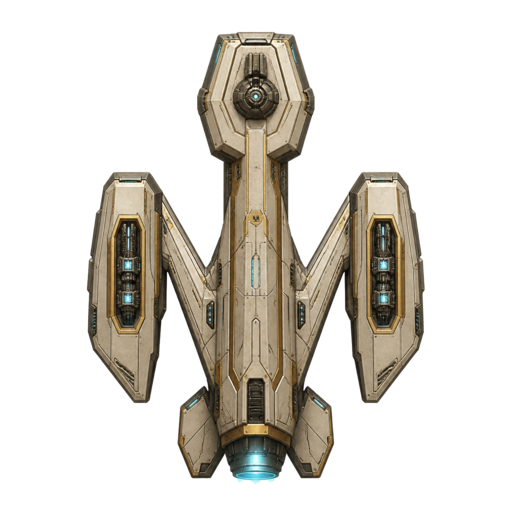
\includegraphics[width=.66in]{../../app/assets/images/ships/tactical/aurelian_frigate.png}};
  \draw[->,reachgold,line width=1.2pt] (0,.30in)--(0,.72in);

  \node[align=center] at (0,-1.78in) {Adjacent arc reference; the frigate's bow points north.\\Each labeled direction continues outward from the ship.};
\end{tikzpicture}
\end{center}

\important{FIRE ONCE}{Each weapon mount may fire only once per turn. Multiple identical mounts shown on a ship are separate weapons and may be fired independently.}
